\begin{figure}[t]
\begin{tabular}{cc}
\begin{subfigure}[b]{0.52\textwidth}
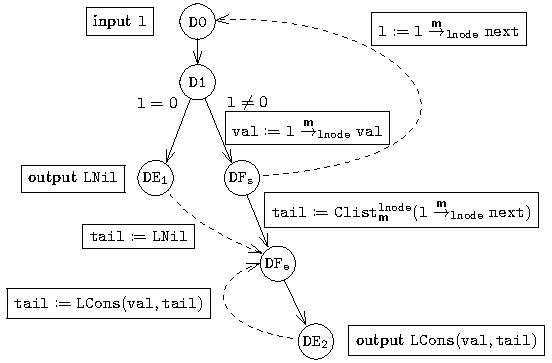
\includegraphics[scale=0.8]{chapters/figures/figClistCfg.pdf}
\vspace{20px}
\caption{\label{fig:reconsProg}Reconstruction Program}
\end{subfigure}%
&
\begin{subfigure}[b]{0.48\textwidth}
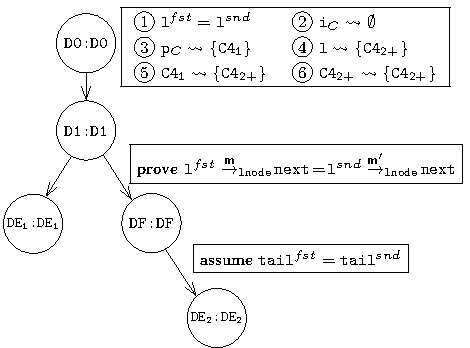
\includegraphics[scale=0.9]{chapters/figures/figClistProductCfg.pdf}
\vspace{20px}
\caption{\label{fig:reconsPCFG}Recons-PCFG}
\end{subfigure}%
%&
%\begin{subfigure}[b]{0.17\textwidth}
%\includegraphics[scale=0.8]{figMallocPointsToGraph.pdf}
%\caption{\label{xxx}XXX}
%\end{subfigure}%
\\
\end{tabular}
\caption{\label{fig:recons}Reconstruction program for \lifted{list}{\mem{}}{lnode}{l} and recons-PCFG between reconstruction programs of \lifted{list}{\mem{}}{lnode}{\cv{l}} and \lifted{list}{\mem{}'}{lnode}{\cv{l}} respectively.
In \cref{fig:reconsProg}, the square boxes show the transfer functions. The dashed edges represent a function call. In \cref{fig:reconsPCFG}, the square box to the right of node (\rrpc{0}{0}) contains the inferred invariants for this recons-PCFG.}
\end{figure}
